% ------ CHAPTER 2 ------

\chapter{Description of the analyzed solution}
% ------ CHAPTER INTRO ------
After the first brief introduction, in this chapter the protocol will be described in detail, showing the so called different \textit{flows} of it, analyzing the exchanged messages, endpoints, tokens management, authorization and finally giving a smattering in mobile applications.
% ------ END OF CHAPTER INTRO ------


% ------ SECTION 2.1 ------
\section{Introduction to the flows}\label{section22}
In a generic use case, when someone has granted permission for an app in order to access his friend list on his behalf, it must happen an interaction between Facebook and the app itself. However, this interaction differs depending on the client natures and capabilities: that is why \textit{\oauth} supports various ways of exchanging information through the use of workflows.
In particular, using the adopted terminology, these are called \textit{grant types} and in the protocol we can find two main grant types that are used in the majority of the cases (the protocol specifies four grant types, but the other two ones are not used in real-world applications):

\begin{itemize}
    \item Implicit grant
    \item Authorization code grant
\end{itemize}

The first one is often cited as the \textbf{client-side workflow}, whereas the second one is often referred to as \textbf{server-side workflow}.
To better understand these two workflows and their purposes, it is significant to underline the concept of \textit{trust} and \textit{user consent}.

% ------ SECTION 2.1.1 ------
\subsection{User consent}
It is clear that when a client application wants to perform a particular action regarding someone or resources someone owns, it must first asks for \textit{permission}. If an App wants to access someone's friends list on Facebook, in order for Facebook to allow this, they must ask directly to the owner. This process may be familiar to many of us. For example, in Fig.~\ref{fig:usercon1} we can see a screenshot of a user consent presented when someone wants to log into Pinterest using the Facebook credentials.

\vspace{0.5cm}
\begin{figure}[htbp]
    \centering
    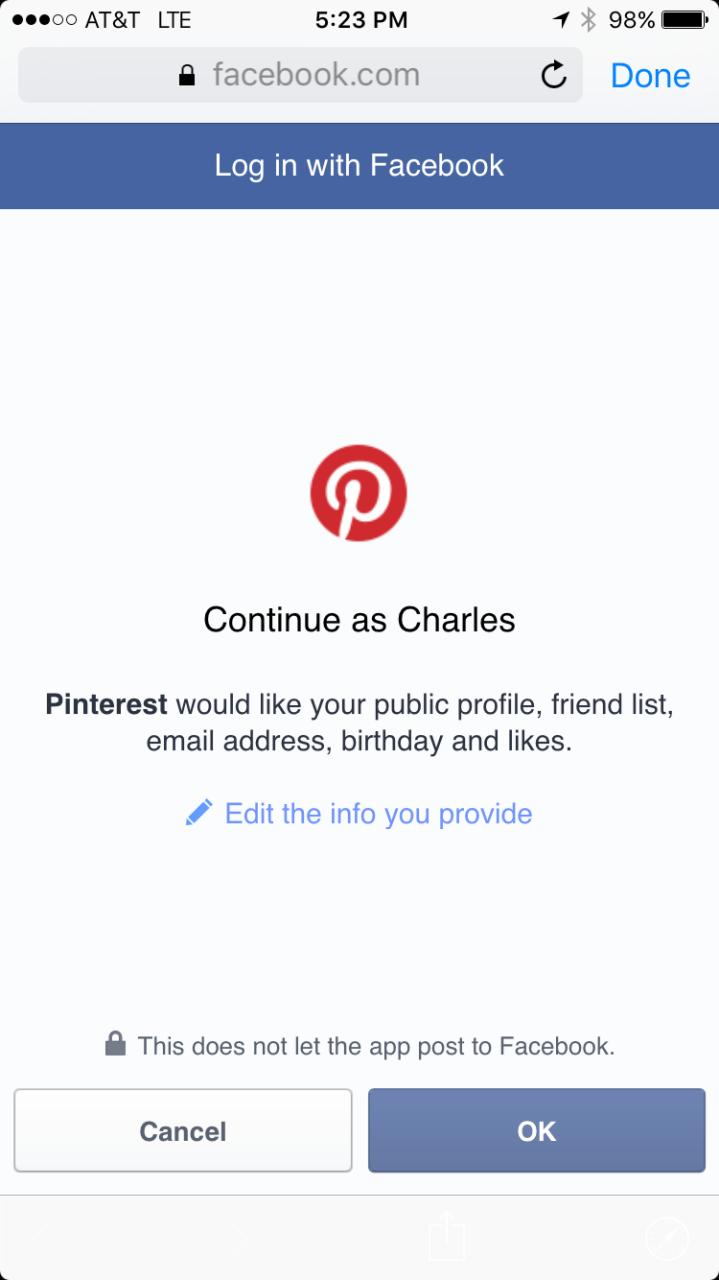
\includegraphics[scale=0.45]{chapters/images/chp2/desktopaccess1.jpg}
    \caption{A classic user consent on Facebook}
    \label{fig:usercon1}
\end{figure}

A first draft of the flowchart sequence is presented in Fig.~\ref{fig:flow1}. The simple steps are:

\begin{enumerate}
    \item The user asks App to suggest contacts.
    \item App says that to be done it needs the authorization here.
    \item App sends the user to Facebook. Here, Facebook asks him directly for authorization for App to access his friend list on his behalf. It does this by presenting the user consent form, which he can either accept or not. Let's assume he accepts.
    \item Facebook happily obliges, giving App the user's friend list. App then uses this information to tailor suggested contacts for him.
\end{enumerate}

However, it is necessary to specifically deal with the distinction of the two grant types in order to better integrate our concepts into a final flowchart.
% ------ END OF SECTION 2.1.1 ------

% ------ SECTION 2.1.2 ------
\subsection{Trusted/Untrusted clients}

In \textit{\oauth} there are only two levels of trust: \textbf{confidential} and \textbf{public}. 
Therefore, a client could be categorized into either of this trust levels following the two simple capabilities of storing and transmitting information securely.

A \textit{trusted client} (\textbf{confidential}) is an application capable of storing and transmitting securely information (credentials, tokens, any other resources necessary for their application).
For example, it could be a 3-tier client-server-DBMS application where the back-end guarantees secure storage and transmission actions for confidential information. 

Instead, an \textit{untrusted client} (\textbf{public}) is one which is incapable of doing such things and so they cannot be trusted on storing/transmitting securely the needed data. All browser-based applications are untrusted clients (HTML/JS) because all the confidential data should be stored in the browser that is absolutely accessible by everyone.
It must be underlined that both capabilities of storing and transmitting must be fulfilled in order to call a client \textit{trusted}.

When the user accepts this form, he has agreed to allow App to access to his Facebook friend list on his behalf. In simple terms, the user has delegated read-only authority to App for his Facebook friend list.
This workflow can be curated some more. There is a very important step in the
preceding process that requires a larger discussion. It is step 4 where App and
Facebook finally exchange the information that has been requested. In the previous diagram, it has been presented as a single step where Facebook gives the information to App. However, in reality, this is a much more complicated exchange that occurs, which depends on many factors. Since this secure and controlled exchange of information is at the crux of what \oauth\ does, it is better to take a closer look.
% ------ END OF SECTION 2.1.2 ------
% ------ END OF SECTION 2.1 ------

\begin{figure}
    \centering
    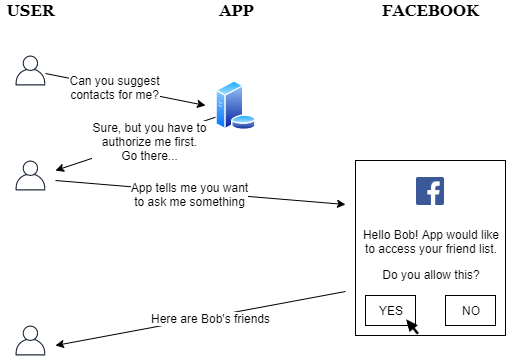
\includegraphics[scale=0.74]{chapters/images/chp2/flow1.png}
    \caption{First draft of the flow}
    \label{fig:flow1}
    \vspace{0.5cm}
\end{figure}

% ------ SECTION 2.2 ------
\section{Token and endpoints management}
Token and endpoints are two important keywords of \textit{\oauth}. In particular, a \textit{token} is an abstraction that replaces that classic \textit{username} and \textit{password} with a single identifier that might have different formats, structures and methods of utilization based on the server that implements it.

Instead, the \textit{endpoints} are crucial for the protocol. In Section 3 of the \rfc{6749}\ specification \cite{RFC6749}, \textit{\oauth} defines three endpoints:

\begin{itemize}
    \item Authorization endpoint
    \item Token endpoint
    \item Redirection endpoint
\end{itemize}

Obviously, not every grant types defines the first two ones.

% ------ SECTION 2.2.1 ------
\subsection{Access and refresh token}
\label{accref}
In \textit{\oauth} two types of token are distinguished.

\textbf{Access token}, that is a very long string that represents the authorization given to the client.

\textbf{Refresh token}, a particular family of tokens used to retrieve a new access token when the current one becomes invalid or expires. They are different from the classic ones because intended to be consumed only with \textit{AuthZ} servers (not resource servers).

% ------ END OF SECTION 2.2.1 ------

% ------ SECTION 2.2.2 ------
\subsection{Authorization and token endpoints}
The \textbf{authorization endpoint} is used by the client to obtain authorization from the resource owner via user-agent redirection (the authorization server must first verify the identity of the resource owner, e.g. using OIDC) and it must use TLS\footnote{Transport Layer Security, "[...] cryptographic protocols designed to provide communications security over a computer network.". Source: \url{https://en.wikipedia.org/wiki/Transport_Layer_Security}} in order to have secure confidential data transmissions.

The \textbf{token endpoint} has the role of waiting for the client in order to return an access token in exchange of an authorization code or a refresh token. That kind of endpoint is not used in the implicit grant type (see section \ref{section22}), because in this case the token is issued directly.
% ------ END OF SECTION 2.2.2 ------

% ------ SECTION 2.3 ------
\section{Client-side flow (untrusted)}
The Implicit Grant flow is optimized for scripting language based clients. As a result of the Resource Owner authorization, the Client is issued an access token directly without issuing an authorization code. This flow is defined in Section 4.2 of the \rfc{6749}\ \cite{RFC6749}. It is important to say that, when using this flow, the authorization server does not authenticate the client (in some cases this could be done via the redirection URI). In this flow, the User-agent is the main actor: it interacts directly with both the User (Resource Owner) and the Client web-app (that is running on it) while sending the necessary messages. In the Fig.~\ref{fig:flowa} is shown a general schema of the flow. The steps follows:

\begin{enumerate}
    \item The User-agent receives the parameters from the Client and redirects the User on the AuthZ Server endpoint with them. The User authenticates and decides whether or not to authorize the Client.
    
    \item If the User authorize it, the AuthZ Server redirects the User back to the redirection URI specified at step 1. The access token is in the URI fragment.
    
    \item The User-agent uses the redirection URI without any URI fragments (the one received with the token is saved locally) to some cloud or local resource of the Client.
    
    \item The returned resource is often a HTML page with an embedded JavaScript code.
    
    \item The User-agent presents the HTML page and runs the embedded script (capable of extracting the access token from the saved URI fragment), delivering the access token to the Client. 
\end{enumerate}

The Implicit Grant flow is much faster and simpler than any other Grant Type and it is well suited for a simple web-app without any back-end server. This flexibility comes with many security issues, starting from the public availability of the access token, that is locally available in the User-agent and it can be extracted by any dangerous script.

\begin{figure}[htbp]
    \centering
    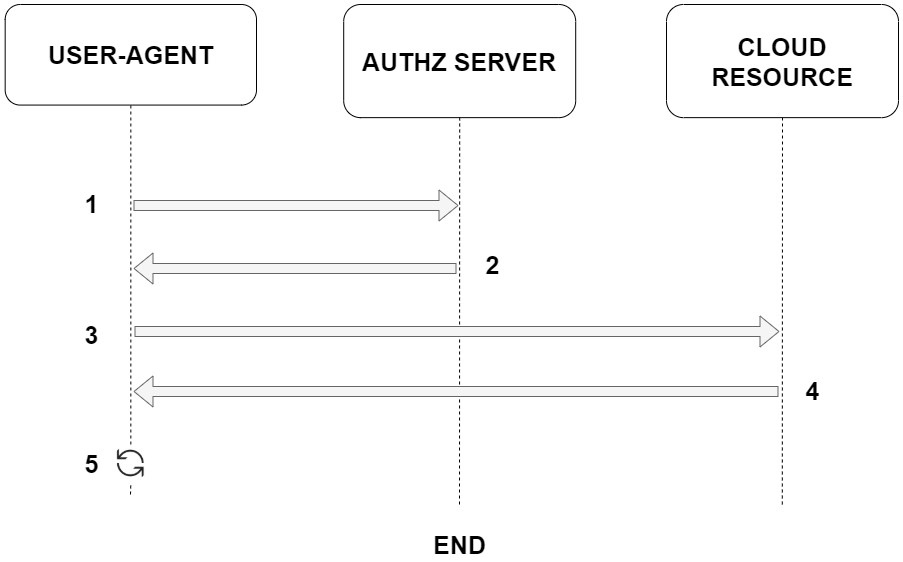
\includegraphics[width=0.9\textwidth]{chapters/images/chp2/implicit_flow_general.png}
    \caption{Implicit Grant flow}
    \label{fig:flowa}
\end{figure}

\vspace{1cm}

% ------ SECTION 2.3.1 ------
\subsection{Analysis of exchanged messages}
At this point, it is clear that for what concerns the Implicit Grant flow we have only an \textbf{authorization request} and an \textbf{access token response}. Both of them must be encoded accordingly to the specification into the endpoint URI in the \textit{application/x-www-form-urlencoded} format.

\subsubsection{Authorization request}
\label{authreq}
With respect to Fig.~\ref{fig:flowa}, the authorization request is done in step 1.
The client MUST build this request using these parameters into the URI fragment:

\texttt{response\_type}

\hspace{0.5cm}REQUIRED. The type has to be \textit{token}.

\texttt{client\_id}

\hspace{0.5cm}REQUIRED. This value must be set with the application's unique client ID.

\texttt{redirect\_uri}

\hspace{0.5cm}OPTIONAL. This value could be set with the URI of the redirection endpoint used by 

\hspace{0.5cm}the service provider to return the response, whether that is an access token in 

\hspace{0.5cm}the case of a successful request, or an error message in the case of a failed request.

\texttt{scope}

\hspace{0.5cm}OPTIONAL. The scope of permissions that we are requesting on behalf of the user.

\vspace{0.5cm}

\texttt{state}

\hspace{0.5cm}RECOMMENDED. String issued by the client in order to maintain a state with

\hspace{0.5cm}the response. Value used by the AuthZ server to redirect the user-agent back to

\hspace{0.5cm}the client.As it will be shown in the following chapters, the param should be

\hspace{0.5cm}used to avoid CSRF\footnote{Cross-site request forgery, "[...] when a malicious program causes a user's web browser to perform an unwanted action on a trusted site on which the user is currently authenticated.". Source: \url{https://auth0.com/docs/protocols/oauth2/mitigate-csrf-attacks}}.

\noindent An example of valid authorization request is:

\begin{lstlisting}[basicstyle=\ttfamily]
  GET /authorize?
    response_type=token&
    client_id=[client_id]&
    redirect_uri=[redirect_uri]&
    scope=[scope]&
    state=[state] HTTP/1.1
  Host: server.example.com
\end{lstlisting}

\subsubsection{Error response}
\label{tokenerr}
For many reasons could happen that the request is not accepted by the resource owner. In this case, an error message is built with those parameters in the fragment of the URI of redirection:

\texttt{error}

\hspace{0.5cm}REQUIRED. Single ASCII code representing the error:

\begin{itemize}
\item[] \begin{itemize}
        \item \texttt{invalid\_request}
        \item \texttt{unauthorized\_client}
        \item \texttt{access\_denied}
        \item \texttt{unsupported\_response\_type}
        \item \texttt{invalid\_scope}
        \item \texttt{server\_error}
        \item \texttt{temporarily\_unavailable}
\end{itemize}
\end{itemize}

\texttt{error\_description}

\hspace{0.5cm}OPTIONAL. Human-readable message describing what caused the error.

\texttt{error\_uri}

\hspace{0.5cm}OPTIONAL. Link to more information about the error.

\texttt{state}

\hspace{0.5cm}REQUIRED. If a state parameter was present in the request.

\vspace{1cm}

\noindent An example of an error response is:

\begin{lstlisting}[basicstyle=\ttfamily]
  HTTP/1.1 302 Found
    Location: [redirect_uri]#
    error=[error_code]&
    error_description=[error_description]&
    error_uri=[error_uri]&
    state=[state]
\end{lstlisting}

\noindent It is important to notice the HTTP 302 Found that redirects to the \texttt{Location} header value. In Fig.~\ref{fig:flowa}, this error response is in step 2.

\subsubsection{Access token response}
When the provider grants the access request, according to the specification it sends a positive response adding to the fragment component of the redirection URI in the \textit{application/x-www-form-urlencoded} format the following parameters:

\texttt{access\_token}

\hspace{0.5cm}REQUIRED. It is this token value that we will eventually use to access

\hspace{0.5cm}the user's profile and feed data.

\texttt{token\_type}

\hspace{0.5cm}REQUIRED. As it suggests, specifies the type of token used

\hspace{0.5cm}to make a protected resource request.

\texttt{expires\_in}

\hspace{0.5cm}RECOMMENDED. The lifetime of the token in seconds. It could not be

\hspace{0.5cm}returned by the server.

\texttt{scope}

\hspace{0.5cm}REQUIRED. The scopes of the access token.

\hspace{0.5cm}OPTIONAL. If they are the same requested by the client.

\texttt{state}

\hspace{0.5cm}REQUIRED. If a state parameter was present in the request.

\noindent An example of an access token response is:

\begin{lstlisting}[basicstyle=\ttfamily]
  HTTP/1.1 302 Found
    Location: [redirect_uri]#
    access_token=[access_token]&
    token_type=[token_type]&
    expires_in=[expires_in]&
    scope=[scope]&
    state=[state]
\end{lstlisting}

\noindent Here too, the HTTP 302 Found redirects to the \texttt{Location} header value without the access token information. As the error response, in Fig.~\ref{fig:flowa} this response is in step 2.

% ------ END OF SECTION 2.3.1 ------
% ------ END OF SECTION 2.3 ------

% ------ SECTION 2.4 ------
\section{Server-side flow (trusted)}
\label{authcg}

The AuthZ Code Grant is the most used Grant Type and it is built for Client confidentiality thanks to the \textit{trusted} capability of a web-server that implements it. The AuthZ Code is delivered by using an AuthZ Server as a broker between Client and Resource Owner. The server authenticates the Resource Owner and obtains authorization before redirecting it back to the Client with the AuthZ Code. This flow is described in Section 4.1 of the \rfc{6749}\ \cite{RFC6749}. It is important to point out that, for this flow, the Resource Owner only authenticates with the authorization server, providing a few important security benefits that will be discussed later on (e.g. client authentication and secure transmission). Moreover, this flow enables the Refresh Token flow that can be used to update the Access Token when it expires, without the Resource Owner intervention. In Fig.~\ref{fig:serverflow} is provided a general description of this flow:

\begin{enumerate}
    \item The flow starts with the Client that builds the URI with the necessary params and redirects the User on the AuthZ Server dedicted endpoint. Here the User logs in and accepts/denies to give authorization to the Client. 
    
    \item If the User accepts, the AuthZ Server redirects the User back to the Client with an AuthZ Code.
    
    \item Without the User intervention, the Client requests the access token by sending the token request with the AuthZ Code to the AuthZ Server.
    
    \item The AuthZ Server sends the access token, and optionally the refresh token. Now the Client can use the access token for accessing resources on a dedicated Resource Server.
\end{enumerate}

\begin{figure}[htbp]
    \centering
    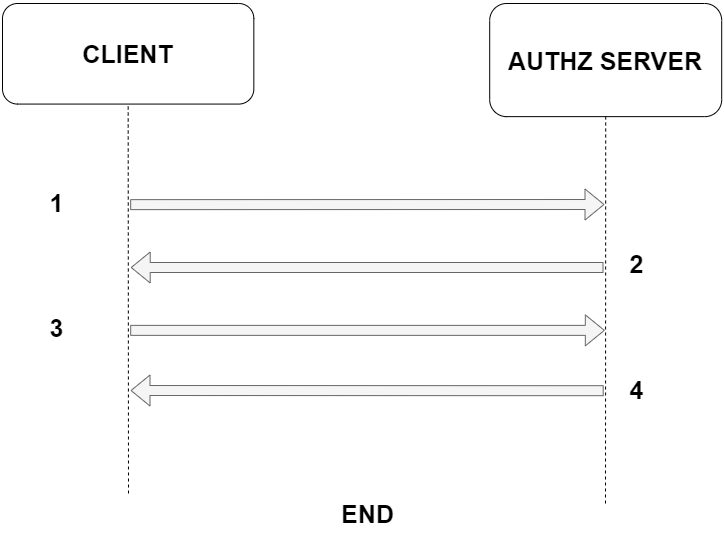
\includegraphics[width=0.9\textwidth]{chapters/images/chp2/server_flow_general.png}
    \caption{Authorization Code Grant flow}
    \label{fig:serverflow}
\end{figure}

With the AuthZ Code Grant flow, since the Client is a \textit{trusted} application capable of storing and transmitting the token securely, some security issues of the Implicit Grant flow disappear. So, naturally, this Client confidentiality comes at a price: complexity. There are twice as much messages exchanged with respect to the Implicit Grant flow, much more libraries to integrate in the code and more parameters to manage. Nevertheless, this is the recommended flow and other flows must be used only in particular cases.


% ------ SECTION 2.4.1 ------
\subsection{Analysis of exchanged messages}
The exchanged messages flow is more complex now. Throughout the AuthZ Code Grant flow, two more messages that precede the token request and response are added: the \textbf{authorization request} and the \textbf{authorization response}. Furthermore, it is suggested the Token Refresh flow use. However, every message must be encoded according to the specification into the URI too using the \textit{application/x-www-form-urlencoded} format.

\subsubsection{Authorization request}
According to the specification, this request is the one to gain consent from the user. This message is nearly identical to the authorization request made in the previous section for the implicit grant flow (\ref{authreq}), except for one important difference: the value of the \texttt{response\_type} parameter MUST be set to \textit{code} instead of \textit{token}.

\noindent This message, with respect to the Fig.~\ref{fig:serverflow}, is exchanged during step 1. An example of valid authorization request is:

\begin{lstlisting}[basicstyle=\ttfamily]
  GET /authorize?
    response_type=code&
    client_id=[client_id]&
    redirect_uri=[redirect_uri]&
    scope=[scope]&
    state=[state] HTTP/1.1
  Host: server.example.com
\end{lstlisting}

\subsubsection{Authorization response}
If the request URL is correctly formatted and constructed, the AuthZ Server will send back a response. If the response will be positive, an authorization code is sent in order to be afterwards converted in an access token.
The possible parameters that can be expected in the preceding response are now in the query component and not in the fragment one:

\texttt{code}

\hspace{0.5cm}REQUIRED. AuthZ code to be exchanged.

\texttt{state}

\hspace{0.5cm}REQUIRED. If a state parameter was present in the request.

\vspace{0.5cm}

\noindent This message, with respect to the Fig.~\ref{fig:serverflow}, is exchanged during step 2. An example of valid authorization resposte is:

\begin{lstlisting}[basicstyle=\ttfamily]
  HTTP/1.1 302 Found
    Location: [redirect_uri]?
    code=[authorization_code]&
    state=[state]
\end{lstlisting}

\vspace{0.5cm}

On the other hand, if the response will be negative, the error will be built as in the Implicit Grant flow (same properties as in \ref{tokenerr}). The difference relies only in the fact that it is returned in the query component instead of the fragment one.

\noindent This message, with respect to the Fig.~\ref{fig:serverflow}, is exchanged during step 2. An example of valid authorization error response is:

\begin{lstlisting}[basicstyle=\ttfamily]
  HTTP/1.1 302 Found
    Location: [redirect_uri]?
    error=[error_code]&
    error_description=[error_description]&
    error_uri=[error_uri]&
    state=[state]
\end{lstlisting}

\subsubsection{Token request}
Once that the authorization code has been retrieved, it can be used to exchange an access token. With this objective, the client makes a request by using a \textit{POST}, specifying in the body section the following parameters:

\texttt{grant\_type}

\hspace{0.5cm}REQUIRED. The value MUST be "authorization\_code".

\texttt{code}

\hspace{0.5cm}REQUIRED. It MUST be set to the value of the previously retrieved

\hspace{0.5cm}authorization code

\texttt{redirect\_uri}

\hspace{0.5cm}REQUIRED. If a redirect\_uri parameter was present in the request.

\texttt{client\_id}

\hspace{0.5cm}REQUIRED. The application unique Client ID.

\vspace{0.5cm}

\noindent This message, with respect to the Fig.~\ref{fig:serverflow}, is exchanged during step 3. An example of valid token request is:

\begin{lstlisting}[basicstyle=\ttfamily]
  POST /token HTTP/1.1
  Host: server.example.com
  Authorization: Basic [base64url_encoded_client_credentials]
  Content-Type: application/x-www-form-urlencoded

  grant_type=authorization_code&
    code=[authorization_code]&
    redirect_uri=[redirect_uri]&
    client_id=[client_id]
\end{lstlisting}

Additionally, in order to pass these parameters to the access token request, the client
application must also identify itself with the service provider. This is an added
layer of security (only necessary for trusted clients) and it is known as \textit{client
authentication}.
It entails the secure transmission of the client credentials to the service provider for validation. It must be pointed out that although the \oauth\ specification doesn't specify any particular authentication scheme for client authentication, this is typically done using HTTP basic authentication [RFC-2617].
In other words, it is the Base64-encoded value of the client credentials in
the form:

    \texttt{BASE64URL([CLIENT\_ID]:[CLIENT\_SECRET])}

\subsubsection{Token response}
As it has been encountered in the previous responses, if the authorization code is valid, we will get our token or an error otherwise. Depending on the implemented server, we could possibly get an optional refresh token (\ref{accref}) in order to update our expired token without doing all the previous steps.

For a \textbf{success} response it is sent back a message with the following parameters in the entity-body (e.g.in JSON):

\texttt{access\_token}

\hspace{0.5cm}REQUIRED. It contains the token: successful authorization and access token request! 

\texttt{token\_type}

\hspace{0.5cm}REQUIRED. Defines the type of token sent.

\hspace{0.5cm}In almost all of the cases this will be \textit{bearer}.

\texttt{expires\_in}

\hspace{0.5cm}RECOMMENDED. The time-to-live of the token.

\hspace{0.5cm}If this value is 7200, that means that the access token will expire

\hspace{0.5cm}two hours from the time the response message was generated.

\vspace{0.5cm}

\texttt{refresh\_token}

\hspace{0.5cm}OPTIONAL. It may be used to refresh the access token in case it expires.

\texttt{scope}

\hspace{0.5cm}REQUIRED. The authorized scopes of the access token.

\hspace{0.5cm}OPTIONAL. If they are the same requested by the client.

\vspace{0.5cm}

\noindent This message, with respect to the Fig.~\ref{fig:serverflow}, is exchanged during step 4. An example of valid token response is:


\begin{lstlisting}[basicstyle=\ttfamily]
  HTTP/1.1 200 OK
  Content-Type: application/json;charset=UTF-8
  Cache-Control: no-store
  Pragma: no-cache
  {
    "access_token":"2YotnFZFEjr1zCsicMWpAA",
    "token_type":"bearer",
    "expires_in":3600,
    "refresh_token":"tGzv3JOkF0XG5Qx2TlKWIA",
  }
\end{lstlisting}

The specification does not provide any information about the type of token, that is why it can be a generic string. Nevertheless, JSON Web Token (JWT) [\rfc{7519}] \cite{RFC7519} is one of the most used. 

% ------ END OF SECTION 2.4.1 ------

% ------ SECTION 2.4.2 ------
\subsection{Refresh Token Flow}
The AuthZ Code Grant flow SHOULD implement the Refresh Token flow. By using the refresh token, the Client (with the AuthZ Server) reduces the User interactions requested by the flow itself:  when the access token expires, the Resource Owner must actively participate to the Code Grant by manually accepting all the authorization requests again and again. In order to avoid this, the refresh token allows to be exchanged with a new access token for the original authorization scopes, reducing the active User interaction only when new authorization scopes are requested. In Fig.~\ref{fig:refreshtok} is shown a the basic flow:

\begin{enumerate}
    \item 
    \item 
    \item 
    \item 
    \item 
    \item 
    \item 
\end{enumerate}

\begin{figure}
    \centering
    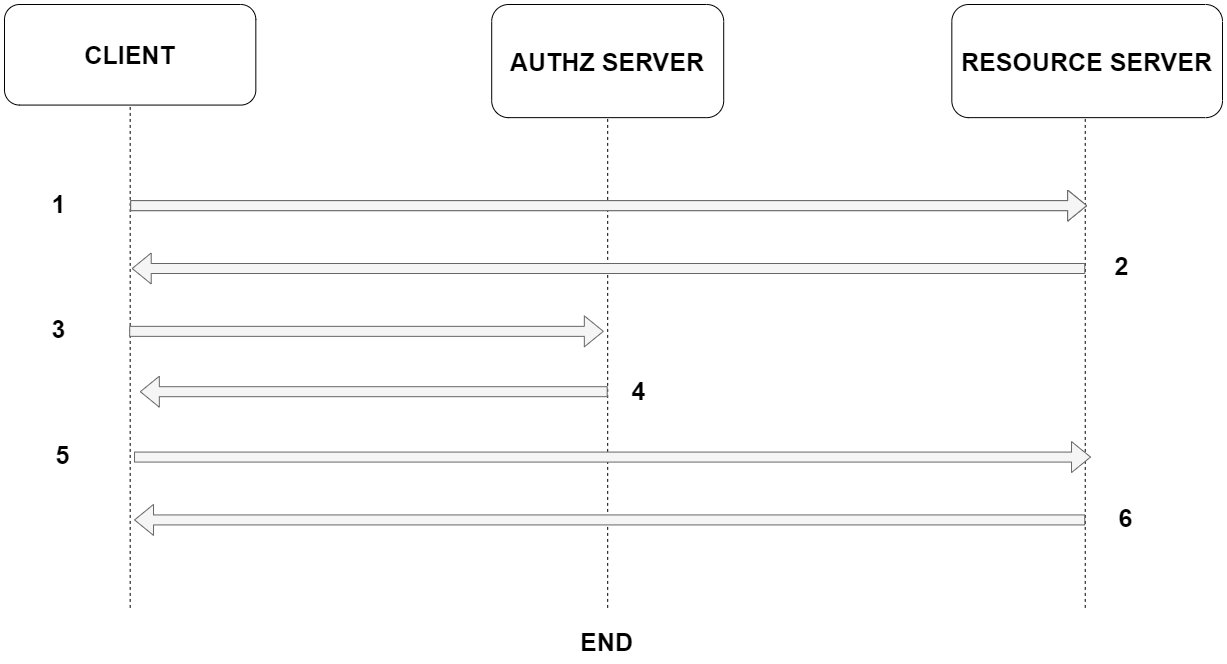
\includegraphics[width=\textwidth]{chapters/images/chp2/refresh_token_general.png}
    \caption{Refresh token flow}
    \label{fig:refreshtok}
\end{figure}
% ------ END OF SECTION 2.4.2 ------
% ------ END OF SECTION 2.4 ------

% ------ SECTION 2.5 ------
\section{About mobile applications}
Typically, when someone talks about \textit{mobile application}, he is referring to one of the two types of applications:

\begin{itemize}
    \item Mobile-optimized web application
    \item Native mobile application
\end{itemize}

The first one is nothing more than a customized browser that runs the web app optimized for the small screen. Since that, the same rules as a desktop web browser are applied.
The second one though, is a natively installed mobile app, an entirely new platform developed in recent years. For this last type, what flow should be used? 

In order to answer this question, just as developing other types of client apps, the flow to be used is based on whether the platform is suitable for being trusted or not. In order for a mobile application to be considered trusted, it must be able to securely store and transmit confidential information. This can really only be achieved in
one way, with the use of a back-end server. If a mobile application has a back-end server that powers it, this server can also be used to securely store and transmit any confidential information it needs to. In this case, yes, this particular type of mobile application can be considered trusted, and should therefore use the authorization code grant flow (as for a web application with a server). 

In the absence of it though, the application will be unable to securely store and transmit confidential information, and cannot be considered trusted. In this scenario, the mobile application should use the implicit grant flow (as for a standalone web app).

% ------ SECTION 2.5.1 ------
\subsection{Secure storage APIs}
It is quite common that not all mobile applications are powered by a back-end server. Rather than use the implicit grant flow, there is a solution that can still archive secure (not strictly) storage capabilities by exploiting secure storage APIs in some mobile platforms like iOS and Android.  For the most part, this is enough for most applications to be considered trusted. Client credentials can be stored here and they can communicate directly with the service provider through the application, accessing these secrets via the APIs without the use of a back-end server.

However, strictly speaking, this is not considered trusted. It is true that the confidential data is encrypted, but it is accessible by the attacker. Data and user/attacker are in the same \textit{space} using this method, while with a back-end server the so called user/attacker space is external with respect to the storage services and not accessible. The platform's secure storage APIs may well be extremely secure and difficult for attackers to break, but in strict terms it is possible and, in the world of security, \textit{possible} should be assumed as \textit{probable}. This is why mobile applications that do not have back-end servers, but make use of the mobile platform's secure storage APIs, should not be considered trusted and should therefore not use the authorization code grant flow.

Since the architecture of the mobile application can be flexible, there is no reason why the application has to use a single authorization workflow. Given a mobile application and a back-end server, it is possible to create a hybrid architecture to leverage the best of both worlds.
% ------ END OF SECTION 2.5.1 ------
% ------ END OF SECTION 2.5 ------

% ------ END OF CHAPTER 2 ------